\documentclass[11pt]{article}
\usepackage[a4paper,margin=26mm,headheight=15pt]{geometry}
\usepackage[T1]{fontenc}
\usepackage{amsmath,amsthm,mathtools}
\usepackage{newpxtext,newpxmath}
\usepackage{microtype}
\usepackage{graphicx,booktabs,array,longtable}
\usepackage[dvipsnames]{xcolor}
\usepackage{enumitem}
\usepackage{fancyhdr}
\usepackage{listings}
\usepackage[most]{tcolorbox}
\usepackage{hyperref}
\usepackage{bookmark}
\definecolor{ink}{HTML}{18384A}
\definecolor{muted}{HTML}{52646E}
\definecolor{pale}{HTML}{F1F5F6}
\hypersetup{colorlinks=true,linkcolor=ink,citecolor=ink,urlcolor=ink,
 pdftitle={Sharp discrepancy for a family of binary substitutions},
 pdfauthor={ChatGPT},pdfsubject={Counterexamples to OEIS A284365 and A284366}}
\pagestyle{fancy}
\fancyhf{}
\fancyhead[L]{\small\textcolor{muted}{Sharp discrepancy for binary substitutions}}
\fancyhead[R]{\small\textcolor{muted}{Research article}}
\fancyfoot[C]{\thepage}
\renewcommand{\headrulewidth}{0.3pt}
\setlength{\parskip}{4pt}
\setlength{\parindent}{1.2em}
\setlength{\emergencystretch}{2em}
\numberwithin{equation}{section}
\newtheorem{theorem}{Theorem}[section]
\newtheorem{lemma}[theorem]{Lemma}
\newtheorem{proposition}[theorem]{Proposition}
\newtheorem{corollary}[theorem]{Corollary}
\theoremstyle{definition}
\newtheorem{definition}[theorem]{Definition}
\theoremstyle{remark}
\newtheorem{remark}[theorem]{Remark}
\newcommand{\N}{\mathbb{N}}
\newcommand{\R}{\mathbb{R}}
\newcommand{\Z}{\mathbb{Z}}
\newcommand{\cl}{\operatorname{cl}}
\newcommand{\sgn}{\operatorname{sgn}}
\newcommand{\eps}{\varepsilon}
\newcommand{\word}{\mathbf{w}}
\newcommand{\OEIS}[1]{\href{https://oeis.org/#1}{\texttt{#1}}}
\lstset{basicstyle=\ttfamily\footnotesize,breaklines=true,columns=fullflexible,
 keepspaces=true,showstringspaces=false,frame=single,rulecolor=\color{muted},
 xleftmargin=4pt,xrightmargin=4pt}
\newtcolorbox{resultbox}{colback=pale,colframe=ink,boxrule=0.5pt,
 arc=1mm,left=3mm,right=3mm,top=2mm,bottom=2mm}
\title{\color{ink}\LARGE Beyond the conjectured bound\\[5pt]
\Large Sharp discrepancy for a family\\of binary substitutions\\[9pt]
\large Counterexamples and corrected theorems for\\OEIS A284365 and A284366}
\author{Research study prepared with ChatGPT}
\date{September 19, 2026}

\begin{document}
\maketitle
\thispagestyle{empty}
\begin{abstract}
The OEIS entries A284365 and A284366 conjecture that two complementary
position sequences associated with the substitution $0\mapsto1$,
$1\mapsto101010$ have linear-approximation errors smaller than $2$.
Both upper bounds are false. Their first counterexamples occur at ranks
$8\,933\,313$ and $2\,977\,771$, respectively, and have the same error
$2.0048721733261288\ldots$. We give exact integer certificates for these
values and for their minimality. More substantially, we determine the
complete discrepancy limit sets for every substitution
$0\mapsto1$, $1\mapsto(10)^m$, $m\ge1$. For the OEIS case $m=3$, the sharp
common upper bound is $(6+\sqrt{21})/5=2.116515138991168\ldots$.
The proof uses two state-dependent prefix-weight intervals and a contracting
set recursion. We also prove the companion density conjectures, construct
explicit infinite families of counterexamples, derive rational generating
functions for their indices, and provide exact-arithmetic random-access
and verification software. The mathematical proofs are self-contained;
finite experiments are supporting checks, not substitutes for the proofs.
\end{abstract}

\begin{resultbox}
\textbf{Status and scope.} The cited OEIS pages still labeled the relevant
statements as conjectures when accessed on September 19, 2026.
This article establishes the stated results by explicit proofs and executed
certificates. It does not claim an exhaustive priority search, peer review,
or proof-assistant formalization. General spectral methods for substitution
discrepancy are classical; the contribution here is the exact solution and
certificates for this family and these particular conjectures.
\end{resultbox}

\clearpage
\tableofcontents
\clearpage

\section{The selected problem and its resolution}\label{sec:problem}

Let $\sigma$ be the substitution
\begin{equation}\label{eq:original-sub}
\sigma(0)=1,\qquad \sigma(1)=101010.
\end{equation}
Its fixed word beginning with $1$ is
\[
\word=101010110101011010101\cdots.
\]
This is \OEIS{A284364} \cite{oeis364}. Number positions starting at $1$.
Let $u(n)$ and $v(n)$ be the positions of the $n$th zero and the $n$th one,
respectively. Thus $u$ is \OEIS{A284365} and $v$ is \OEIS{A284366}
\cite{oeis365,oeis366}. Put
\begin{equation}\label{eq:rs3}
r=\frac{9+\sqrt{21}}6,\qquad
s=\frac{\sqrt{21}-1}2,\qquad \frac1r+\frac1s=1.
\end{equation}
The position-sequence entries conjecture
\begin{equation}\label{eq:conjectures}
-2<rn-u(n)<2,\qquad -1<sn-v(n)<2\qquad(n\ge1).
\end{equation}
They also conjecture their respective densities to be
$(9-\sqrt{21})/10$ and $(1+\sqrt{21})/10$. The density comments are dated
April 13, 2025; the sequence entries credit Clark Kimberling, March 26,
2017. We use the unambiguous position-sequence formulations: the parent
entry's comment uses count terminology alongside position slopes, which
would be a different and immediately incompatible statement.

\begin{theorem}[Resolution for the OEIS sequences]\label{thm:original}
Write $E_0(n)=rn-u(n)$ and $E_1(n)=sn-v(n)$. For every $n\ge1$,
\begin{align}
-\frac{12+2\sqrt{21}}{15}&<E_0(n)<\frac{6+\sqrt{21}}5,\label{eq:zero3}\\
\frac{\sqrt{21}-9}{5}&<E_1(n)<\frac{6+\sqrt{21}}5.\label{eq:one3}
\end{align}
Each endpoint is a subsequential limit, and indeed the full set of
subsequential limits of each error sequence is the corresponding closed
interval. In particular, both conjectured lower bounds in
\eqref{eq:conjectures} hold, but both upper bounds fail infinitely often.

The first counterexamples are
\begin{equation}\label{eq:first-values}
v(2\,977\,771)=5\,334\,043,\qquad
u(8\,933\,313)=20\,222\,898.
\end{equation}
Their common error is
\begin{equation}\label{eq:common-error}
\frac{2\,977\,771\sqrt{21}-13\,645\,857}{2}
=2.00487217332612884794005732278\ldots>2.
\end{equation}
The two asserted densities are correct.
\end{theorem}

The bounds are not consequences of extrapolating the observed maxima.
Sections~\ref{sec:family}--\ref{sec:positions} prove them for an entire
family. Section~\ref{sec:certificate} supplies a finite certificate for
\eqref{eq:first-values} and its minimality. Section~\ref{sec:infinite}
gives an explicit sequence of errors increasing to the sharp upper
endpoint. The method belongs to the established study of the relation
between substitution spectra and discrepancy \cite{adamczewski}; all
specific interval and sharpness arguments needed here are proved below.

\section{A parameterized family and its discrepancy theorem}\label{sec:family}

Fix an integer $m\ge1$ and define
\begin{equation}\label{eq:family-sub}
\sigma_m(0)=1,\qquad \sigma_m(1)=(10)^m.
\end{equation}
The image of $1$ begins with $1$ and has length at least $2$, so the words
$\sigma_m^k(1)$ form nested prefixes of an infinite fixed word
$\word^{(m)}$. The substitution contains both letters in an iterate of
either letter; no additional initial condition is needed beyond the
initial $1$.

Throughout the general argument let
\begin{equation}\label{eq:parameters}
q=\frac{\sqrt{m^2+4m}-m}{2},\quad
\lambda=m+q=\frac mq,\quad
s=1+q,\quad r=1+\frac1q,
\end{equation}
and
\begin{equation}\label{eq:CH}
t=1-q,\qquad C=\frac{q}{1-q^2},\qquad
H=qC=\frac{q^2}{1-q^2}.
\end{equation}
The quantities depend on $m$, even when the subscript is suppressed.
The following identities will be used repeatedly:
\begin{equation}\label{eq:identities}
0<q<1,\quad q^2=m(1-q),\quad
q(1+H)=C,\quad H(1+q)=m,\quad
\frac1r+\frac1s=1.
\end{equation}
For example, $H(1+q)=q^2/(1-q)=m$. Also $q$ is irrational:
$(m+1)^2<m^2+4m<(m+2)^2$ for $m\ge1$.

Let $Z(N)$ and $O(N)$ count the zeros and ones in the first $N$ letters,
with $Z(0)=O(0)=0$. Let $u_m(n)$ and $v_m(n)$ denote the corresponding
position sequences, and set
\[
E_0(n)=rn-u_m(n),\qquad E_1(n)=sn-v_m(n).
\]

\begin{theorem}[Sharp error intervals for every $m$]\label{thm:general}
For every integer $m\ge1$ and $n\ge1$,
\begin{align}
C-m&<E_1(n)<C,\label{eq:general-one}\\
\frac{1-C}{q}&<E_0(n)<C.\label{eq:general-zero}
\end{align}
The closures of the two error-value sets are exactly these intervals
with their endpoints included. These are also their full subsequential
limit sets. No endpoint is attained at a finite index.

For every $N\ge0$,
\begin{equation}\label{eq:general-density}
-\frac{H}{1+q}<O(N)-\frac{N}{1+q}<\frac{C}{1+q}.
\end{equation}
Again, the two endpoints are sharp, and the closure of the centered
counting errors is the full closed interval. In particular,
\[
\lim_{N\to\infty}\frac{O(N)}N=\frac1s,\qquad
\lim_{N\to\infty}\frac{Z(N)}N=\frac1r.
\]
\end{theorem}

A useful equivalent form of the lower zero-position endpoint is
\begin{equation}\label{eq:zero-lower-alt}
\frac{1-C}{q}=C-1-\frac{m-1}{q}.
\end{equation}
For $m=3$, substituting $q=(\sqrt{21}-3)/2$ gives
\[
C=\frac{6+\sqrt{21}}5,\qquad
H=\frac{3+3\sqrt{21}}{10},
\]
and \eqref{eq:general-one}--\eqref{eq:general-zero} become
\eqref{eq:one3}--\eqref{eq:zero3}.

\section{A contracting weight and two prefix states}\label{sec:weight}

For a finite binary word $P$, define its weight by
\begin{equation}\label{eq:weight}
X(P)=|P|_0-q|P|_1.
\end{equation}
This is additive under concatenation. The incidence matrix of the
substitution, with row order $0,1$ and column order $0,1$, is
\[
M=\begin{pmatrix}0&m\\1&m\end{pmatrix}.
\]
Its eigenvalues are $\lambda$ and $-q$. More directly, the letter weights
give the identity on which the proof rests:
\begin{lemma}[Weight contraction]\label{lem:contraction}
For every finite word $P$,
\begin{equation}\label{eq:weight-contract}
X(\sigma_m(P))=-qX(P).
\end{equation}
\end{lemma}
\begin{proof}
For $P=0$ the two sides equal $-q$. For $P=1$, the image has $m$ letters
of each type and hence weight $m(1-q)=q^2=-q(-q)$. Additivity proves the
claim for an arbitrary concatenation of letters.
\end{proof}

The next letter is crucial. For $a\in\{0,1\}$, let
\begin{equation}\label{eq:state-def}
S_a=\{X(w_1\cdots w_N):N\ge0,\ w_{N+1}=a\}.
\end{equation}
Thus $0\in S_1$, from the empty prefix. A prefix ending immediately
before a zero belongs to state $0$, not to a state determined by its last
letter.

\begin{lemma}[Exact state equations]\label{lem:state}
The sets in \eqref{eq:state-def} satisfy
\begin{align}
S_0&=\bigcup_{j=0}^{m-1}(-qS_1+jt-q),\label{eq:state0}\\
S_1&=(-qS_0)\ \cup\!
\bigcup_{j=0}^{m-1}(-qS_1+jt).\label{eq:state1}
\end{align}
\end{lemma}
\begin{proof}
View the fixed word as the concatenation of images of its own letters.
If a parent prefix $P$ is followed by $0$, its image is followed by the
single letter $1$, giving the transition $-qS_0$ in \eqref{eq:state1}.
If $P$ is followed by $1$, its image is followed by $(10)^m$.
Immediately before the $(j+1)$st one in that image, the internal prefix is
$(10)^j$, whose weight is $jt$. Immediately before the corresponding
zero, the internal prefix is $(10)^j1$, whose weight is $jt-q$.
Lemma~\ref{lem:contraction} gives all the stated affine images.
Conversely, every location in the fixed word lies in one of these image
blocks. Thus there are no missing transitions and the equations are
set equalities.
\end{proof}

Using a single state and adding all possible offsets independently would
forget which parent letter permits which offset. The two-state system
retains precisely the information required for the sharp constants.

\section{Solving the interval recursion, including sharpness}\label{sec:intervals}

Define two closed intervals
\begin{equation}\label{eq:intervals}
I_0=[-C,H-1],\qquad I_1=[-qH,H].
\end{equation}
They are nondegenerate for every $m\ge1$.

\begin{lemma}[Invariant intervals]\label{lem:intervals}
The pair $(I_0,I_1)$ satisfies \eqref{eq:state0}--\eqref{eq:state1}
with $S_a$ replaced by $I_a$.
\end{lemma}
\begin{proof}
Put $J_j=-qI_1+jt$. Each $J_j$ has length
\[
qH(1+q)=mq,
\]
while successive left endpoints are separated by $t=1-q=q^2/m$.
If $m\ge2$, then $mq\ge t$, so adjacent intervals overlap. For $m=1$
there is only one interval. The extreme endpoints yield
\begin{equation}\label{eq:unionJ}
\bigcup_{j=0}^{m-1}J_j=[-qH,H-t].
\end{equation}
Indeed, the upper endpoint is $q^2H+(m-1)t=H-t$, since
$q^2(H+1)=H$ and $mt=q^2$.

Subtracting $q$ from \eqref{eq:unionJ} gives
\[
\bigcup_{j=0}^{m-1}(J_j-q)=[-qH-q,H-t-q]=[-C,H-1]=I_0.
\]
For state $1$, the other image is
\[
-qI_0=[q-qH,H].
\]
It overlaps or touches the interval in \eqref{eq:unionJ}, because
\[
H-t\ge q-qH
\quad\Longleftrightarrow\quad H(1+q)\ge1
\quad\Longleftrightarrow\quad m\ge1.
\]
Their union is therefore $[-qH,H]=I_1$.
\end{proof}

\begin{lemma}[Strict inclusion of all actual prefixes]\label{lem:strict}
Every element of $S_a$ lies in the interior of $I_a$.
\end{lemma}
\begin{proof}
We induct on the length $N$ of the prefix. The empty prefix has weight
$0$, which lies strictly inside $I_1$.

For a nonempty prefix, locate its next letter in an image block. The
associated parent prefix has some length $k<N$. To see strict decrease,
if $k>0$ then that parent prefix begins with $1$, so its image has length
at least $k+(2m-1)>k$; this image is contained in the original prefix.
If $k=0$, strict decrease follows from $N>0$.

By induction, the parent weight belongs to the interior of its appropriate
interval. Its actual transition is an affine map with nonzero slope
$-q$. The image of an interior point is an interior point of the image
interval, and Lemma~\ref{lem:intervals} puts that image interval inside
the appropriate target interval. Such a point cannot be an endpoint of
the target interval. This completes the induction.
\end{proof}

Bounds alone do not prove sharpness. We next show that the intervals
contain no gap in the closures of the actual prefix weights.

\begin{lemma}[Uniqueness for the compact set recursion]\label{lem:hausdorff}
Let $K_0,K_1$ be nonempty compact subsets of $\R$ satisfying the state
equations. Then $K_0=I_0$ and $K_1=I_1$.
\end{lemma}
\begin{proof}
For compact nonempty subsets of $\R$, write $d_H$ for Hausdorff distance.
An affine map of slope $-q$ multiplies this distance by $q$.
Also, for finite indexed families,
\[
d_H\left(\bigcup_i A_i,\bigcup_i B_i\right)
\le\max_i d_H(A_i,B_i).
\]
Let $D=\max\{d_H(K_0,I_0),d_H(K_1,I_1)\}$. Apply these observations to
the two state equations for $K$ and $I$. They imply $D\le qD$.
Since $D$ is finite and $0<q<1$, it follows that $D=0$.
\end{proof}

\begin{proposition}[Exact closures]\label{prop:closures}
\begin{equation}\label{eq:closures}
\cl S_0=[-C,H-1],\qquad \cl S_1=[-qH,H].
\end{equation}
The closure of all prefix weights is $[-C,H]$.
\end{proposition}
\begin{proof}
Lemma~\ref{lem:strict} makes $S_0,S_1$ bounded, and both are nonempty.
Take closures in their exact finite-union equations. Closure commutes
with each affine map and with a finite union, so $(\cl S_0,\cl S_1)$ is
a compact fixed pair. Lemma~\ref{lem:hausdorff} proves \eqref{eq:closures}.
Finally $I_0$ and $I_1$ overlap or touch, since
$H-1\ge-qH$ is again equivalent to $m\ge1$. Their union is $[-C,H]$.
\end{proof}

Distinct prefix lengths have distinct weights. Indeed, equality would
give $\Delta Z=q\Delta O$, impossible for irrational $q$ unless both
integer differences vanish, in which case the lengths agree. A set dense
in a nondegenerate interval has infinitely many distinct points in every
relative neighborhood of every point of that interval. Consequently its
density statements remain valid after deleting any finite number of
prefixes. This proves that the closures just obtained are also the full
sets of limits along prefix lengths tending to infinity.

\section{Position errors, densities, and exact transfer}\label{sec:positions}

\subsection{Passing from prefix weights to position errors}
Immediately before the $n$th one, the prefix has $n-1$ ones and
$v_m(n)-n$ zeros. Its weight is therefore
\begin{equation}\label{eq:weight-one}
X=v_m(n)-n-q(n-1)=q-E_1(n).
\end{equation}
Immediately before the $n$th zero, the prefix has $n-1$ zeros and
$u_m(n)-n$ ones, giving
\begin{equation}\label{eq:weight-zero}
X=n-1-q(u_m(n)-n)=qE_0(n)-1.
\end{equation}
Apply the strict state bounds and Proposition~\ref{prop:closures}.
Equation~\eqref{eq:weight-one} transforms $I_1$ into
\[
[q-H,q+qH]=[C-m,C],
\]
and \eqref{eq:weight-zero} transforms $I_0$ into
$[(1-C)/q,C]$. The identities follow from \eqref{eq:identities}.
The state sets contain exactly the prefixes immediately before the
respective ranked letters, so no additional selection restriction is
needed. This proves the position part of Theorem~\ref{thm:general},
including strictness and the full subsequential limit sets.

For ordinary prefix counts,
\begin{equation}\label{eq:count-weight}
X=N-(1+q)O(N),\qquad
O(N)-\frac{N}{1+q}=-\frac{X}{1+q}.
\end{equation}
The total prefix-weight interval $[-C,H]$ proves
\eqref{eq:general-density} and its sharpness. Dividing the bounded
counting error by $N$ establishes the densities without invoking an
ergodic theorem. In the case $m=3$, this yields the quantitative estimate
\begin{equation}\label{eq:density3}
-\frac{33+3\sqrt{21}}{50}
<O(N)-\frac{1+\sqrt{21}}{10}N
<\frac{27+7\sqrt{21}}{50}.
\end{equation}
Thus the density conjectures in all three relevant OEIS entries follow,
and the error in the unnormalized counting function is uniformly bounded.

\subsection{A relation between the two position sequences}
\begin{proposition}[Exact position transfer]\label{prop:transfer}
For $n\ge1$ and $1\le h\le m$,
\begin{equation}\label{eq:transfer}
u_m(m(n-1)+h)=v_m(n)+(2m-1)n-2m+2h.
\end{equation}
Equivalently,
\begin{equation}\label{eq:error-transfer}
E_0(m(n-1)+h)=E_1(n)-(m-h)(r-2).
\end{equation}
In particular,
\begin{equation}\label{eq:mn}
u_m(mn)=v_m(n)+(2m-1)n,\qquad E_0(mn)=E_1(n).
\end{equation}
\end{proposition}
\begin{proof}
Before the parent word's $n$th one there are $n-1$ ones and
$v_m(n)-n$ zeros. The total length of their images is
$2m(n-1)+v_m(n)-n$. The image of the next one contains $m$ zeros, at
internal positions $2,4,\ldots,2m$, and no zero comes from the image of a
parent zero. Thus the $h$th such zero has global rank $m(n-1)+h$ and the
position in \eqref{eq:transfer}.

Subtract this expression from $r(m(n-1)+h)$. The identity
$m(r-2)=q$ reduces the result to \eqref{eq:error-transfer}.
\end{proof}

For $m=3$, $C<r$; explicitly
\[
r-C=\frac{9-\sqrt{21}}{30}>0.
\]
Since $r-2>0$, \eqref{eq:error-transfer} shows that the errors at
zero ranks $3(n-1)+1$ and $3(n-1)+2$ are strictly less than
$C-(r-2)<2$. It follows that
\begin{equation}\label{eq:violations-bijection}
\{k:E_0(k)>2\}=\{3n:E_1(n)>2\}.
\end{equation}
Equality to $2$ is impossible, because $r$ and $s$ are irrational.
This bijection will make the zero-position minimality result immediate
once the first one-position violation has been certified.

\section{An exact finite certificate and the first counterexamples}\label{sec:certificate}

\subsection{Recursive blocks}
Define auxiliary finite words
\begin{equation}\label{eq:blocks}
W_{-1}=0,\quad W_0=1,\quad
W_k=(W_{k-1}W_{k-2})^m\quad(k\ge1).
\end{equation}
For $k\ge0$, induction gives $W_k=\sigma_m^k(1)$. In particular,
$W_k$ is a prefix of $\word^{(m)}$. Write $L_k,Z_k,O_k$ for its length,
zero count, and one count. Each satisfies
\begin{equation}\label{eq:block-recurrence}
a_k=m(a_{k-1}+a_{k-2}).
\end{equation}
For the remainder of this section $m=3$.

Consider the finite word
\begin{equation}\label{eq:P-witness}
P=W_{11}\,W_{10}\,W_{10}\,W_8\,W_6\,W_4\,W_2.
\end{equation}
This is a prefix of $W_{12}$, followed by a $1$. Here is an explicit
way to follow the recursive decomposition. In
$W_{12}=(W_{11}W_{10})^3$, take the first $W_{11}W_{10}$, then enter the
next $W_{11}=(W_{10}W_9)^3$ and take its first $W_{10}$. The residual
word begins with $W_9$. In $W_9=(W_8W_7)^3$, take $W_8$, leaving a word
beginning with $W_7$. Repeat with $W_7,W_5,W_3$, taking $W_6,W_4,W_2$.
The remaining word begins with $W_1=101010$, so its next letter is $1$.

The count recurrence gives
\begin{equation}\label{eq:P-counts}
|P|_0=2\,356\,272,\quad |P|_1=2\,977\,770,\quad
|P|=5\,334\,042.
\end{equation}
Consequently the next one proves the first identity in
\eqref{eq:first-values}. Formula~\eqref{eq:mn} proves the second:
\[
u(3\cdot2\,977\,771)=5\,334\,043+5\cdot2\,977\,771
=20\,222\,898.
\]
Their common error is exactly \eqref{eq:common-error}.
To certify that it exceeds $2$, it suffices to observe
\begin{equation}\label{eq:square-certificate}
21(2\,977\,771)^2-(13\,645\,861)^2=265\,940>0.
\end{equation}
Both quantities compared before squaring are positive, so
\eqref{eq:square-certificate} proves
$2\,977\,771\sqrt{21}>13\,645\,861$ with no numerical approximation.

\subsection{Why no earlier index is a counterexample}
For any finite word $U$, define
\[
\mu_1(U)=\min\{X(Q): Q\text{ is a proper prefix of }U,
\text{ and the next letter in }U\text{ is }1\}.
\]
Use $+\infty$ if $U$ has no one. For concatenations,
\begin{align}
\mu_1(UV)&=\min\{\mu_1(U),X(U)+\mu_1(V)\},\label{eq:min-concat}\\
\mu_1(B^m)&=\mu_1(B)+\min\{0,(m-1)X(B)\}.\label{eq:min-power}
\end{align}
The second formula follows by considering the $m$ translated copies of
$B$. These identities give a small exact certificate for all earlier
positions at once.

\begin{table}[htbp]
\centering\small
\begin{tabular}{rrrrl}
\toprule
$k$ & $L_k$ & $Z_k$ & $O_k$ & $\mu_1(W_k)$\\
\midrule
0&1&0&1&$0$\\
1&6&3&3&$0$\\
2&21&9&12&$6-8q$\\
3&81&36&45&$9-12q$\\
4&306&135&171&$99-126q$\\
5&1\,161&513&648&$144-183q$\\
6&4\,401&1\,944&2\,457&$1\,440-1\,821q$\\
7&16\,686&7\,371&9\,315&$2\,088-2\,640q$\\
8&63\,261&27\,945&35\,316&$20\,718-26\,184q$\\
9&239\,841&105\,948&133\,893&$30\,033-37\,956q$\\
10&909\,306&401\,679&507\,627&$297\,819-376\,374q$\\
11&3\,447\,441&1\,522\,881&1\,924\,560&$431\,712-545\,583q$\\
12&13\,070\,241&5\,773\,680&7\,296\,561&$4\,280\,832-5\,409\,957q$\\
\bottomrule
\end{tabular}
\caption{Block data for $m=3$. Every minimum is calculated by
\eqref{eq:min-concat}--\eqref{eq:min-power}, using exact quadratic-field
comparisons. The $k=12$ row is included for context; only the preceding
rows are needed to certify $P$.}\label{tab:blocks}
\end{table}

Apply \eqref{eq:min-concat} to the seven factors of $P$. The translated
candidate minima, in their order of appearance, are
\begin{equation}\label{eq:seven-minima}
\begin{aligned}
&431\,712-545\,583q,&&1\,820\,700-2\,300\,934q,\\
&2\,222\,379-2\,808\,561q,&&2\,346\,957-2\,965\,998q,\\
&2\,355\,624-2\,976\,951q,&&2\,356\,227-2\,977\,713q,\\
&2\,356\,269-2\,977\,766q.&&
\end{aligned}
\end{equation}
Their minimum is the first, so
\begin{equation}\label{eq:muP}
\mu_1(P)=431\,712-545\,583q.
\end{equation}
All of these finite comparisons can be checked by the integer sign rule
in Section~\ref{sec:algorithms}; the separate checker in the archive
recomputes the block table and its minimum rather than accepting them as
input.

By \eqref{eq:weight-one}, the largest one-position error strictly before
the candidate equals
\begin{equation}\label{eq:prior-max}
q-\mu_1(P)=545\,584q-431\,712
=1.988978393507077166\ldots<2.
\end{equation}
The last inequality has the exact certificate
\begin{equation}\label{eq:prior-square}
(2\,500\,180)^2-21(545\,584)^2=110\,224>0.
\end{equation}
It proves $545\,584\sqrt{21}<2\,500\,180$, which is precisely
\eqref{eq:prior-max}$<2$ after substituting the value of $q$.
The maximum in \eqref{eq:prior-max} occurs at rank $545\,584$, at
position $977\,296$.

Every earlier ranked one lies in $P$. Hence no earlier one-position error
is at least $2$. Equations~\eqref{eq:square-certificate} and
\eqref{eq:prior-square} certify the first counterexample, and the exact
bijection \eqref{eq:violations-bijection} certifies the first zero-position
counterexample. This proof covers all earlier indices; it is not a claim
based only on a finite sample of selected positions.

\section{Infinite extremal families and their generating functions}\label{sec:infinite}

The compact-set proof gives sharpness nonconstructively in terms of
closures. A specific family approaching the common upper endpoint can
also be written down and evaluated by short recurrences.

\begin{proposition}[Explicit extremal prefixes]\label{prop:extremal}
For general $m\ge1$, let $P_0$ be the empty word and define
\begin{equation}\label{eq:extremal-prefix}
P_{j+1}=\sigma_m^2(P_j)(10)^m,\qquad U_j=\sigma_m(P_j).
\end{equation}
Every $P_j$ and every $U_j$ is a prefix of the fixed word, followed by a
$1$. Set
\begin{equation}\label{eq:extremal-np}
n_j=|U_j|_1+1,\qquad p_j=|U_j|+1.
\end{equation}
Then
\begin{equation}\label{eq:extremal-errors}
v_m(n_j)=p_j,\qquad
E_1(n_j)=C(1-q^{2j+2})\nearrow C.
\end{equation}
The zero-position errors at ranks $mn_j$ are equal to these errors.
\end{proposition}
\begin{proof}
Suppose $P_j$ is a prefix followed by $1$. Its image is followed by
$(10)^m$. Therefore $\sigma_m(P_j)1$ is a prefix followed by $0$.
Apply the substitution again: the resulting prefix is
$\sigma_m^2(P_j)(10)^m=P_{j+1}$, followed by $\sigma_m(0)=1$.
This proves the prefix assertion inductively from $P_0$. It also shows
that $U_j$ is followed by $1$.

By Lemma~\ref{lem:contraction} and $m(1-q)=q^2$,
\[
X(P_{j+1})=q^2X(P_j)+q^2.
\]
Starting at zero and summing the geometric progression gives
$X(P_j)=H(1-q^{2j})$. Thus
\[
E_1(n_j)=q-X(U_j)=q+qH(1-q^{2j})
=C-Cq^{2j+2},
\]
where $q+qH=C$ and $qH=Cq^2$. The errors increase strictly because
$0<q<1$. The zero-position assertion follows from \eqref{eq:mn}.
\end{proof}

Let $(z_j,o_j)=(|P_j|_0,|P_j|_1)$. The preceding construction is fully
integer-recursive:
\begin{equation}\label{eq:counts-extremal}
\begin{pmatrix}z_{j+1}\\o_{j+1}\end{pmatrix}
=\begin{pmatrix}m&m^2\\m&m^2+m\end{pmatrix}
\begin{pmatrix}z_j\\o_j\end{pmatrix}
+\begin{pmatrix}m\\m\end{pmatrix},\qquad (z_0,o_0)=(0,0),
\end{equation}
with
\begin{equation}\label{eq:np-fromcounts}
n_j=z_j+mo_j+1,\qquad p_j=z_j+2mo_j+1.
\end{equation}
Eliminating the two counts yields an especially simple result.

\begin{corollary}[Scalar recurrences and rational generating functions]
\label{cor:gf}
Put $T=m(m+2)$. Then
\begin{align}
n_{j+2}&=Tn_{j+1}-m^2n_j+1-m,
& n_0&=1,& n_1&=m^2+m+1,\label{eq:nrec}\\
p_{j+2}&=Tp_{j+1}-m^2p_j+m^2-m+1,
& p_0&=1,& p_1&=2m^2+m+1.\label{eq:prec}
\end{align}
Their ordinary generating functions are
\begin{align}
\sum_{j\ge0}n_jz^j
&=\frac{1-mz}{(1-z)(1-m(m+2)z+m^2z^2)},\label{eq:ngf}\\
\sum_{j\ge0}p_jz^j
&=\frac{1+m(m-1)z}{(1-z)(1-m(m+2)z+m^2z^2)}.\label{eq:pgf}
\end{align}
\end{corollary}
\begin{proof}
The linear part in \eqref{eq:counts-extremal} is $M^2$, with trace
$T$ and determinant $m^2$. Its characteristic identity implies the two
inhomogeneous recurrences after substitution in \eqref{eq:np-fromcounts};
alternatively, one may eliminate $z_j,o_j$ directly. The constant terms
and initial values follow by evaluating $j=0,1,2$.

For a sequence obeying $a_{j+2}=Ta_{j+1}-m^2a_j+c$, multiplying its
series by $1-Tz+m^2z^2$ gives
$a_0+(a_1-Ta_0)z+cz^2/(1-z)$. For \eqref{eq:nrec}, the numerator after
multiplication by $1-z$ reduces to $1-mz$; for \eqref{eq:prec}, it reduces
to $1+m(m-1)z$. This proves both generating functions.
\end{proof}

\begin{table}[htbp]
\centering\small
\begin{tabular}{rrrr}
\toprule
$j$ & $n_j$ & $p_j=v(n_j)$ & $E_1(n_j)$, rounded\\
\midrule
0&1&1&0.791287847478\\
1&13&22&1.286742017213\\
2&184&328&1.596963935937\\
3&2\,641&4\,729&1.791205189187\\
4&37\,957&67\,990&1.912826719410\\
5&545\,584&977\,296&1.988978393507\\
6&7\,842\,145&14\,047\,537&2.036659732964\\
7&112\,721\,917&201\,917\,398&2.066514757944\\
8&1\,620\,249\,448&2\,902\,333\,144&2.085208077525\\
\bottomrule
\end{tabular}
\caption{An explicit extremal family for $m=3$. It supplies infinitely many
counterexamples, but its first violation ($j=6$) is not the first violation
over all ranks.}\label{tab:family}
\end{table}

In the OEIS case the recurrences are
$n_{j+2}=15n_{j+1}-9n_j-2$ and
$p_{j+2}=15p_{j+1}-9p_j+7$. Formula~\eqref{eq:extremal-errors} shows
that every $j\ge6$ gives a counterexample. The closed-interval theorem is
stronger still: every open interval contained in $(2,C)$ contains infinitely
many errors of each position sequence, not just those in this special
family.

\subsection{Exact asymptotics along the extremal family}
The denominator in \eqref{eq:ngf}--\eqref{eq:pgf} factors as
\[
(1-z)(1-\lambda^2z)(1-q^2z).
\]
Here $\lambda>1$ and $0<q<1$, so partial fractions give an exact
three-term expansion. For either sequence $a_j=n_j$ or $a_j=p_j$, let
\[
d=\frac{c}{1-2m},\quad
A=\frac{a_1-d-q^2(a_0-d)}{\lambda^2-q^2},\quad B=a_0-d-A,
\]
where $c$ is the corresponding constant in its recurrence. Then
\begin{equation}\label{eq:exact-expansion}
a_j=A\lambda^{2j}+d+Bq^{2j}.
\end{equation}
The leading coefficient is positive, as follows either from these
expressions or the positive count recurrence. In particular,
$n_j,p_j=\Theta(\lambda^{2j})$, whereas
\begin{equation}\label{eq:gap-rate}
C-E_1(n_j)=Cq^{2j+2}=\Theta(p_j^{-\kappa}),\qquad
\kappa=-\frac{\log q}{\log\lambda}.
\end{equation}
For $m=3$, $\kappa=0.17565278149\ldots$. This is a statement along the
constructed subsequence, not a claim about the optimal record-error
convergence rate over every prefix. The comparatively small exponent
explains why substantial growth in the rank can coexist with a slow
approach to the limiting extremum.

\section{Exact algorithms and executed checks}\label{sec:algorithms}

\subsection{Quadratic arithmetic without rounding decisions}
Every prefix weight and every one-position error is of the form $a+bq$
with integer $a,b$. Since $q^2=m-mq$, addition and multiplication stay
in this representation. To compare $a+bq$ with zero, put
\[
A=2a-mb,\qquad D=m^2+4m.
\]
Its sign is the sign of $A+b\sqrt D$. If $A$ and $b$ have the same
nonzero sign, that sign is the answer. Zero cases are immediate. If
they have opposite signs, the answer is
\begin{equation}\label{eq:sign-rule}
\sgn(A)\,\sgn(A^2-Db^2).
\end{equation}
As $D$ is nonsquare, there is no unhandled nontrivial equality case.
Thus all block-extremum decisions and counterexample inequalities in the
software reduce to integer arithmetic. Zero-position errors may contain
$1/q$; multiplying their comparisons by the positive number $q$ puts
them in the same representation.

\subsection{Associative summaries and random access}
A block summary stores its zero and one counts, and for each following
letter state the minimum and maximum prefix weight, together with a
location attaining the extremum. Under concatenation $UV$, the extrema
from $V$ are translated by $X(U)$ and their positions by $|U|$; the
appropriate minimum or maximum is then taken with the extrema from $U$.
This is the same identity as \eqref{eq:min-concat} in both states and
both directions.

Precompute summaries for $W_{-1},W_0,\ldots,W_k$ using
\eqref{eq:blocks}. To count the first $N$ letters, find the first block
long enough, skip whole child pairs by their lengths, and descend into
the residual child. To find the $n$th specified letter, use its block
counts instead of lengths. At a fixed $m$, there are $O(\log N)$ levels,
and each level involves only a bounded number of arithmetic operations.
The library groups repeated child pairs for these operations.

To find the first error at least a threshold $B$, a block beginning after
a prefix of weight $x$ can be discarded exactly when its appropriate
extremum cannot reach the threshold. For ones the feasibility condition is
\[
x+\mu_1(W_k)\le q-B.
\]
For zeros, using the maximum prefix weight $\nu_0(W_k)$ before a zero,
the condition is
\[
x+\nu_0(W_k)\ge qB-1.
\]
Find a first feasible enclosing block, then inspect children from left to
right and descend into the first feasible child, skipping the others by
their counts. The returned leaf is the first violation, and the skipped
block extrema certify that no earlier one was missed.

For fixed $m$ and a counterexample at a position of size $N$, the
precomputation and descent use $O(\log N)$ arithmetic operations on
$O(\log N)$-bit integers. This is an arithmetic-operation count, not a
unit-cost bit-complexity assertion. With $\mathsf M(b)$ denoting the cost
of multiplying $b$-bit integers, the sign tests give the conservative
bound $O(\log N\,\mathsf M(\log N))$ bit operations, alongside additions
and small-parameter divisions. Storing all summaries uses
$O((\log N)^2)$ bits at fixed $m$. Searching only up to a prescribed
level and finding nothing is a finite negative result, not a proof of
nonexistence in the infinite word.

\subsection{What was actually checked}
The delivered script \texttt{code/verify.py --long} completed successfully
under Python 3.13.5. It recorded $310\,816$ explicit checks, in addition
to the assertions internal to the separate certificate checker.
For every $m=1,\ldots,8$, it built a literal $12\,000$-letter prefix,
checked the sharp bounds at every letter, and compared selected random-access
queries and complete small-block extrema against direct calculations.
It also checked the transfer identity, the exact extremal family through
$j=24$, and the proposed recurrences and generating-function numerators.

For $m=3$, the script compared the first $30$ displayed terms of each
position sequence and the first $30$ binary letters with the OEIS entries.
It did not download or compare the complete linked $10\,000$-term tables.
The optional long test independently formed the fixed-word prefix of
length $20\,222\,898$ by literal substitution, confirming both specified
counterexample positions and ranks. The first-counterexample search used
exact summaries, not a floating-point scan.

The file \texttt{code/independent\_check.py} does not import the main
library. It reconstructs the count and minimum certificate with a
separate integer sign test and concatenation implementation. This checks
the finite computations supporting minimality; the prefix-membership
argument and transfer theorem supply their mathematical justification.
The verification data in \texttt{data/} records exact coefficients as
well as display decimals, and includes the full first-violation descent
traces. No experiment is used to infer the infinite interval theorem.

\begin{figure}[htbp]
\centering
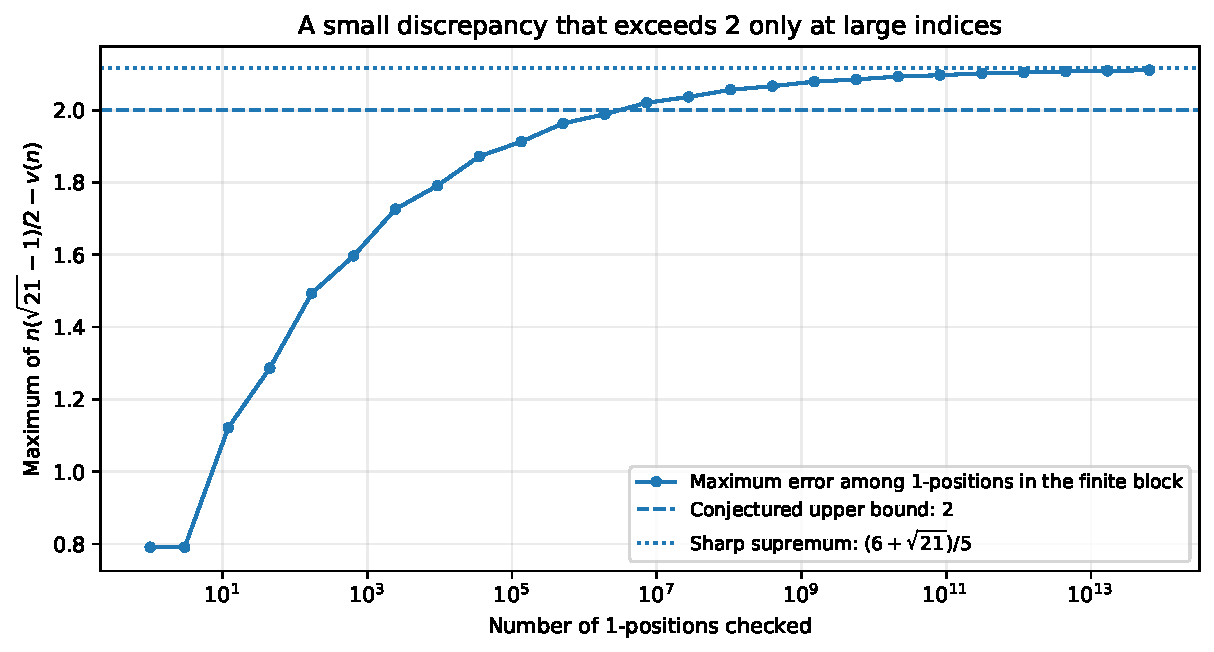
\includegraphics[width=\linewidth]{figures/finite_maxima.pdf}
\caption{Maximum one-position error over all ones in $W_k$, for
$k=0,\ldots,24$. The horizontal scale is the number of one-positions in
the enclosing block, not the rank at which its maximum is attained.
The curve is computed from exact block summaries; floating-point values
are used only to render the figure.}\label{fig:maxima}
\end{figure}

\section{Further consequences and boundaries of the result}\label{sec:consequences}

\subsection{The \texorpdfstring{$m=1$}{m=1} endpoint is a Beatty pair}
At $m=1$, $q=(\sqrt5-1)/2$ and $C=1$. Both error intervals become
$(0,1)$. Since the positions are integers and the slopes are irrational,
\[
v_1(n)=\lfloor(1+q)n\rfloor,\qquad
u_1(n)=\left\lfloor\left(1+\frac1q\right)n\right\rfloor.
\]
Thus the familiar complementary Beatty description is recovered directly
from the theorem. For $m\ge2$, no fixed real shift $\gamma$ can give
$v_m(n)=\lfloor sn+\gamma\rfloor$ for every $n$: such an expression would
put all its errors in an interval of length $1$, whereas the error
closure in \eqref{eq:general-one} has length exactly $m$. The density
already forces any putative Beatty slope to be $s$.

\subsection{A finite factor-balance bound}
The centered prefix-counting errors have range width
\[
\frac{C+H}{1+q}=C.
\]
For a factor of length $L$, its number of ones minus $L/s$ is the
difference of two prefix errors, so it lies strictly between $-C$ and
$C$. Two factors of the same length consequently differ in their numbers
of ones by an integer whose absolute value is strictly less than $2C$.
Hence
\begin{equation}\label{eq:balance-bound}
\bigl||A|_1-|B|_1\bigr|\le\lceil2C\rceil-1
\qquad\text{whenever }|A|=|B|.
\end{equation}
For $m=3$ this gives a balance bound of $4$. The article does not assert
that this bound is optimal: sharp prefix extrema do not automatically
occur at two endpoints separated by the same prescribed factor length.
The exact optimal factor-balance constant is a separate question.

\subsection{The word itself has a nonrational generating function}
Although the extremal-index series \eqref{eq:ngf}--\eqref{eq:pgf} are
rational, the characteristic series
\[
F_m(z)=\sum_{n\ge1}w^{(m)}_n z^n
\]
is not rational. Indeed, a rational power series has coefficients obeying
an eventual fixed linear recurrence. If those coefficients take values
in a finite set, the vector of a fixed number of consecutive coefficients
has only finitely many states and deterministically produces its successor.
A state eventually repeats, making the sequence eventually periodic.
An eventually periodic binary sequence has rational density, contradicting
$1/(1+q)$, which is irrational. This elementary observation concerns the
full word, not the rational generating functions of the sparse families.

\subsection{What remains outside the claims}
The conjectured upper bounds and density statements selected in
Section~\ref{sec:problem} are resolved by the preceding proofs. The
article does not determine the frequency distribution of discrepancy
values within their interval, the density of the ranks with error above
$2$, or the exact best factor-balance constant. Knowing the support of
subsequential limits does not by itself answer those distributional
questions. Nor is the constructed extremal subsequence claimed to enumerate
all record errors. These distinctions prevent stronger statements from
being inferred merely from the observed finite data or the interval
closure result.

\section{Conclusion}
A conjecture about an error below $2$ can survive a substantial finite
check while failing only slightly at a much larger index. Here the first
one-position violation occurs at rank $2\,977\,771$, and its transfer
produces the first zero-position violation at rank $8\,933\,313$.
The finite disproof is certified by a short recursive prefix and two
integer square comparisons. The structural analysis goes further: the
correct common upper bound is $(6+\sqrt{21})/5$, and a two-state contraction
proves exact discrepancy intervals for every $0\mapsto1$,
$1\mapsto(10)^m$. Density, explicit extremal families, rational
index-generating functions, and efficient exact verification then follow
from the same framework.

\clearpage
\appendix
\section{Reproducing and inspecting the deliverables}\label{app:reproduce}

All verification code uses only the Python standard library and requires
Python 3.10 or later. From the archive's top-level directory run:
\begin{lstlisting}
python code/independent_check.py
python code/verify.py --long
\end{lstlisting}
The shorter command \texttt{python code/verify.py} omits the
$20$-million-letter literal construction but retains the exact
first-counterexample search and finite certificate. A successful run
writes its own report and regenerates the exact data. Running the shorter
command will replace the saved report with one that accurately records
that the long test was omitted.

For an individual large-index query:
\begin{lstlisting}[language=Python]
from substitution import Substitution

model = Substitution(3)
assert model.select(1, 2977771) == 5334043
assert model.select(0, 8933313) == 20222898
print(model.first_at_least(1, threshold=2))
\end{lstlisting}
Run this from \texttt{code/}, or add that directory to the Python module
search path. Ranks and returned positions are $1$-based; prefix lengths
and internal offsets are $0$-based. The exact search's \texttt{None}
result means that no witness was found through the specified maximum
block level, not that the infinite sequence has no witness.

The main archive components are described in Table~\ref{tab:files}.
The pre-rendered figure is included, so compiling the article does not
require Python or Matplotlib. To rebuild the PDF, run \texttt{pdflatex}
on \texttt{article.tex} twice; the bibliography is embedded in the source.
To rebuild only the plot, run \texttt{python code/make\_figure.py}, which
requires Matplotlib. No fonts, checksum files, temporary TeX build files,
or downloaded copies of other authors' papers are included.

\begin{table}[htbp]
\centering\small
\begin{tabular}{p{0.40\linewidth}p{0.53\linewidth}}
\toprule
File or directory & Purpose\\
\midrule
\texttt{article.tex}, \texttt{article.pdf} & Complete source and compiled article.\\
\texttt{code/substitution.py} & Exact quadratic arithmetic, summaries, counts, selection, first-threshold search.\\
\texttt{code/independent\_check.py} & Separate compact checker for the finite certificate.\\
\texttt{code/verify.py} & Executable cross-checks and data generation.\\
\texttt{data/certificates.json} & First-counterexample traces and exact certificate coefficients.\\
\texttt{data/finite\_extrema.json} & Block extrema through $W_{30}$.\\
\texttt{data/extremal\_family.json} & First $25$ explicit extremal-family terms.\\
\texttt{data/verification.json} & Report of the executed test suite.\\
\texttt{figures/} & The figure in vector PDF and raster PNG form.\\
\texttt{oeis\_proposed\_updates.txt} & Suggested mathematical corrections, not submitted to OEIS.\\
\texttt{README.md} & Build instructions, scope, and verification notes.\\
\bottomrule
\end{tabular}
\caption{Archive contents.}\label{tab:files}
\end{table}

\clearpage
\phantomsection
\addcontentsline{toc}{section}{References}
\begin{thebibliography}{9}
\bibitem{oeis364}
The OEIS Foundation Inc., \emph{A284364: Fixed point of the morphism
$0\mapsto1$, $1\mapsto101010$}. Entry credited to Clark Kimberling,
March 26, 2017; density conjecture comment by Amiram Eldar, April 13, 2025.
\url{https://oeis.org/A284364}. Accessed September 19, 2026.

\bibitem{oeis365}
The OEIS Foundation Inc., \emph{A284365: Positions of 0 in A284364;
complement of A284366}. Entry credited to Clark Kimberling,
March 26, 2017; density conjecture comment by Amiram Eldar, April 13, 2025.
\url{https://oeis.org/A284365}. Accessed September 19, 2026.

\bibitem{oeis366}
The OEIS Foundation Inc., \emph{A284366: Positions of 1 in A284364;
complement of A284365}. Entry credited to Clark Kimberling,
March 26, 2017; density conjecture comment by Amiram Eldar, April 13, 2025.
\url{https://oeis.org/A284366}. Accessed September 19, 2026.

\bibitem{adamczewski}
B.~Adamczewski, \emph{Symbolic discrepancy and self-similar dynamics},
Annales de l'Institut Fourier \textbf{54} (2004), no.~7, 2201--2234.
\href{https://doi.org/10.5802/aif.2079}{doi:10.5802/aif.2079}.
\url{https://www.numdam.org/item/AIF_2004__54_7_2201_0/}.
\end{thebibliography}
\end{document}
